
\documentclass[aspectratio=169]{beamer}
\usetheme{Madrid}
\usecolortheme{default}

\usepackage{amsmath,amsfonts,amssymb}
\usepackage{graphicx}
\usepackage{tikz}
\usepackage{pgfplots}
\pgfplotsset{compat=1.18}
\usepackage{bm}

% ---------- helpers ----------
\newcommand{\nvec}{\hat{\mathbf{n}}}
\newcommand{\lvec}{\hat{\mathbf{l}}}
\newcommand{\vvec}{\hat{\mathbf{v}}}
\newcommand{\rvec}{\hat{\mathbf{r}}}
\newcommand{\hvec}{\hat{\mathbf{h}}}
\newcommand{\clamp}{\mathrm{max}}
\newcommand{\Hemisphere}{\Omega^+}

% tidy lists and footer
\let\olditem\item
\renewcommand{\item}{\olditem \vspace{2pt}}
\setbeamertemplate{navigation symbols}{}

% ---------- title ----------
\title{Importance Sampling in BRDF Evaluation}
\subtitle{Advanced Monte Carlo Techniques for Realistic Rendering}
\author{Team : Z\_Buffer : 2005076, 2005106, 2005110}
\institute{BUET CSE 409: Computer Graphics}
\date{\today}

\begin{document}

% === Frame 1: Title ===
\begin{frame}
  \titlepage
  \begin{center}
    \vspace{0.4cm}
    \textcolor{blue}{\large Exploratory Presentation on Advanced Graphics Topics}
  \end{center}
\end{frame}

% === Frame 2: Rendering challenge ===
\begin{frame}{The Rendering Challenge (Why sampling?)}
\begin{columns}
\begin{column}{0.58\textwidth}
\textbf{Goal:} Compute outgoing light toward the camera.

\medskip
\textbf{Rendering equation (single bounce):}
\[
L_o(\vvec)=\int_{\Hemisphere} f_r(\lvec,\vvec)\,L_i(\lvec)\,(\nvec\!\cdot\!\lvec)\,\mathrm{d}\lvec
\]

\textbf{Why sample?}
\begin{itemize}
  \item Light can come from any direction on the hemisphere.
  \item Exact integration is rarely possible.
  \item Use \textbf{Monte Carlo}: estimate with random samples.
\end{itemize}
\end{column}
\begin{column}{0.42\textwidth}
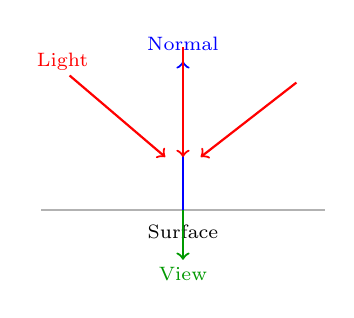
\begin{tikzpicture}[scale=0.9, every node/.style={font=\scriptsize}]
  % Surface
  \draw[thick, gray!60] (-2,-0.5) -- (2,-0.5);
  \node at (0,-0.8) {Surface};

  % Normal
  \draw[->, thick, blue] (0,-0.5) -- (0,1.6);
  \node[blue] at (0,1.85) {Normal};

  % Incoming light
  \draw[->, red, thick] (-1.6,1.4) -- (-0.25,0.25);
  \draw[->, red, thick] ( 1.6,1.3) -- ( 0.25,0.25);
  \draw[->, red, thick] ( 0.0,1.8) -- ( 0.0,0.25);
  \node[red] at (-1.7,1.6) {Light};

  % View
  \draw[->, thick, green!60!black] (0,-0.5) -- (0,-1.2);
  \node[green!60!black] at (0,-1.4) {View};
\end{tikzpicture}
\end{column}
\end{columns}
\end{frame}

% === Frame 3: BRDF basics ===
\begin{frame}{BRDF: the surface's reflection rule}
\begin{columns}
\begin{column}{0.54\textwidth}
\textbf{BRDF} $f_r(\lvec,\vvec)$ says: given incoming direction $\lvec$ and view direction $\vvec$, how much light is reflected?

\medskip
\textbf{Three simple specular models (non–IS):}
\begin{align*}
\textbf{Phong:}\quad & f_r=\clamp(\rvec\!\cdot\!\vvec,0)^n,\quad \rvec=\text{reflect}(-\lvec,\nvec)\\
\textbf{Blinn--Phong:}\quad & f_r=\clamp(\nvec\!\cdot\!\hvec,0)^n,\quad \hvec=\frac{\lvec+\vvec}{\|\lvec+\vvec\|}\\
\textbf{Cook--Torrance:}\quad & f_r \propto D(\theta)\,F(\theta)\,G(\theta)
\end{align*}

\textbf{Meaning:}
\begin{itemize}
  \item $n$ = shininess (larger $n$ \(\Rightarrow\) tighter highlight).
  \item $D$ = microfacet distribution, $F$ = Fresnel, $G$ = geometry (shadowing/masking).
\end{itemize}
\end{column}
\begin{column}{0.46\textwidth}
\begin{tikzpicture}[scale=0.8, every node/.style={font=\scriptsize}]
  % Surface
  \draw[thick, gray!60] (-2.6,-0.5) -- (2.6,-0.5);
  \node at (0,-0.85) {Surface};

  % Normal
  \draw[->, thick, blue] (0,-0.5) -- (0,1.9);
  \node[blue] at (0,2.1) {Normal};

  % Specular lobes
  \draw[red, thick, fill=red!18] (0,-0.5) -- (0.65,1.45) -- (-0.65,1.45) -- cycle;        % Phong
  \draw[green!60!black, thick, fill=green!18] (0,-0.5) -- (0.45,1.2) -- (-0.45,1.2) -- cycle; % Blinn-Phong
  \draw[blue, thick, fill=blue!18] (0,-0.5) -- (0.28,0.95) -- (-0.28,0.95) -- cycle;          % Cook-Torrance

  % Legend boxed (left)
  \begin{scope}
    \coordinate (L) at (-2.55,1.95);
    \draw[rounded corners=2pt, gray!40] ($(L)+(-0.15,-1.05)$) rectangle ($(L)+(2.15,0.15)$);
    \node[anchor=west] at (L) {\footnotesize \bfseries Specular lobe width:};
    \node[anchor=west] at ($(L)+(0,-0.35)$) {\textcolor{red}{\large$\bullet$}\;Phong (widest)};
    \node[anchor=west] at ($(L)+(0,-0.65)$) {\textcolor{green!60!black}{\large$\bullet$}\;Blinn--Phong (medium)};
    \node[anchor=west] at ($(L)+(0,-0.95)$) {\textcolor{blue}{\large$\bullet$}\;Cook--Torrance (narrowest)};
  \end{scope}
\end{tikzpicture}
\end{column}
\end{columns}
\end{frame}

% === Frame 4: Monte Carlo ===
\begin{frame}{Monte Carlo: estimating the integral}
\textbf{Integral:}\quad
\[
I=\int_{\Hemisphere} f(\omega)\,\mathrm{d}\omega
\quad \approx \quad
\frac{1}{N}\sum_{i=1}^N \frac{f(\omega_i)}{p(\omega_i)}
\qquad (\omega_i \sim p)
\]

\medskip
\begin{columns}
\begin{column}{0.5\textwidth}
\textbf{Uniform}
\[
p(\omega)=\frac{1}{2\pi}\ \ (\text{hemisphere})
\]
Simple but wastes samples where $f$ is small.
\end{column}
\begin{column}{0.5\textwidth}
\textbf{Importance sampling}
\[
p(\omega)\propto f(\omega)
\]
More samples where contribution is large $\Rightarrow$ less noise, faster.
\end{column}
\end{columns}
\end{frame}

% === Frame 5: Importance sampling (simple forms) ===
\begin{frame}{Importance Sampling PDFs (simple, slide-ready)}
\textbf{1) Phong}
\[
\boxed{\,f_r^{\text{Phong}}(\theta_R)=\cos^n(\theta_R)\,},\qquad
\boxed{\,p_{\text{Phong}}(\theta_R)=\frac{n+1}{2\pi}\cos^n(\theta_R)\,}
\]
Sampling: \(\theta_R=\arccos\!\big(u_1^{1/(n+1)}\big),\ \phi=2\pi u_2\).

\medskip
\textbf{2) Blinn--Phong}
\[
\boxed{\,f_r^{\text{Blinn-Phong}}(\theta_H)=\cos^n(\theta_H)\,},\qquad
\boxed{\,p_{\text{Blinn-Phong}}(\theta_H)=\frac{n+1}{2\pi}\cos^n(\theta_H)\,}
\]
Sampling: \(\theta_H=\arccos\!\big(u_1^{1/(n+1)}\big),\ \phi=2\pi u_2\).

\medskip
\textbf{3) Cook--Torrance (microfacet)}
\[
\boxed{\,f_r^{\text{Cook-Torrance}}(\theta)\ \propto\ D(\theta)\,F(\theta)\,G(\theta)\,},\qquad
\boxed{\,p_{\text{Cook-Torrance}}(\theta)\ \propto\ D(\theta)\,\cos\theta\,}
\]
Pick a distribution \(D\) (e.g., GGX or Beckmann) and normalize over the hemisphere.
\end{frame}

% === Frame 6: Variables (kept simple) ===
\begin{frame}{Variables (quick guide)}
\begin{columns}
\begin{column}{0.62\textwidth}
\begin{itemize}
  \item $\nvec$ – surface normal (up direction at the point).
  \item $\lvec$ – incoming light direction.
  \item $\vvec$ – view (camera) direction.
  \item $\rvec$ – perfect mirror reflection of $-\lvec$ about $\nvec$.
  \item $\hvec$ – halfway direction between $\lvec$ and $\vvec$.
  \item $\theta_R$ – angle to the reflection direction $\rvec$ (Phong).
  \item $\theta_H$ – angle to the halfway direction $\hvec$ (Blinn–Phong).
  \item $\theta$ – angle from the normal (used in microfacet $D(\theta)$).
  \item $n$ – shininess exponent (higher $n$ = tighter highlight).
  \item $D,F,G$ – microfacet distribution, Fresnel, geometry terms.
  \item $u_1,u_2$ – uniform random numbers in $[0,1)$ for sampling.
\end{itemize}
\end{column}
\begin{column}{0.38\textwidth}
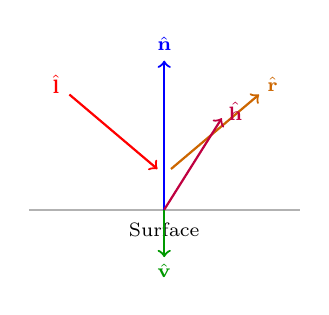
\begin{tikzpicture}[scale=0.86, every node/.style={font=\scriptsize}]
  % Surface
  \draw[thick, gray!60] (-2,-0.5) -- (2,-0.5);
  \node at (0,-0.8) {Surface};

  % Normal
  \draw[->, thick, blue] (0,-0.5) -- (0,1.7);
  \node[blue] at (0,1.95) {$\nvec$};

  % l, v, r, h
  \draw[->, thick, red] (-1.4,1.2) -- (-0.1,0.1); \node[red] at (-1.6,1.35) {$\lvec$};
  \draw[->, thick, green!60!black] (0,-0.5) -- (0,-1.2); \node[green!60!black] at (0,-1.4) {$\vvec$};
  \draw[->, thick, orange!80!black] (0.1,0.1) -- (1.4,1.2); \node[orange!80!black] at (1.6,1.35) {$\rvec$};
  \draw[->, thick, purple] (0,-0.5) -- (0.85,0.85); \node[purple] at (1.05,0.95) {$\hvec$};
\end{tikzpicture}
\end{column}
\end{columns}
\end{frame}

% === Frame 7: Why IS helps ===
\begin{frame}{Why importance sampling reduces noise}
\[
L_o \approx \frac{1}{N}\sum_{i=1}^N
\frac{f_r(\lvec_i,\vvec)\,L_i(\lvec_i)\,(\nvec\!\cdot\!\lvec_i)}{p(\lvec_i)}
\]
If $p(\omega)$ is large where $f_r(\omega)$ is large, the ratio is stable $\Rightarrow$ lower variance and faster convergence.
\end{frame}

% === Frame 8: Tiny implementation hint (optional) ===
\begin{frame}{Implementation hint}
\begin{itemize}
  \item Build a local frame aligned to the axis you sample around (reflection for Phong, normal for Blinn/Cook).
  \item Convert $(\theta,\phi)$ to a direction in the local frame, then rotate to world.
  \item Always clamp dot products with $\max(\cdot,0)$.
\end{itemize}
\end{frame}

% === Frame 9: When to use which ===
\begin{frame}{When to use which}
\begin{columns}
\begin{column}{0.5\textwidth}
\textbf{Phong / Blinn–Phong}
\begin{itemize}
  \item Simple highlights, teaching, previews.
  \item IS PDF: $\dfrac{n+1}{2\pi}\cos^n(\cdot)$.
\end{itemize}
\end{column}
\begin{column}{0.5\textwidth}
\textbf{Cook–Torrance}
\begin{itemize}
  \item Modern PBR look (metals, roughness).
  \item IS PDF: $p(\theta)\propto D(\theta)\cos\theta$ (normalize).
\end{itemize}
\end{column}
\end{columns}
\end{frame}

% === Frame 10: Conclusion ===
\begin{frame}{Conclusion}
\begin{itemize}
  \item Importance sampling = sample more where the BRDF is strong.
  \item Use the simple PDFs shown for each model.
  \item Keep variables straight: $\theta_R$ (Phong), $\theta_H$ (Blinn), $D(\theta)$ for Cook–Torrance.
\end{itemize}
\end{frame}

\end{document}

